\section{Aggregate LHS Method(Same Solution Parameters)}

This solution was calculated using the same solution input arguments as the Stochastic Loads method. The command line that was used was:

\begin{verbatim}
python -m pystruct <<data_file>>  -S2 -i80 -g200 --csv
\end{verbatim}

\noindent Where: 

\begin{itemize}
  \item \codeword{-S2}: Select solution 2: Aggregate LHS method
  \item \codeword{-i80}: Use a population size of 80. 
  \item \codeword{-g200}: Use a generation count of 200. 
  \item \codeword{--csv}: Generate CSV output for final Pareto Front
\end{itemize}

\subsection{Resultant Pareto Front}
Table \ref{tab:pfront_agg_sameparam} shows the design parameters of the members of the Pareto Front generated by this solution run. The Pareto Front is also given graphically in Figure \ref{fig:pfront_agg_sameparam}. 
\begin{table}[!htbp]
\small
\begin{tabular}{|p{1.5cm}p{1.5cm}p{1.5cm}p{1.4cm}p{2cm}p{2cm}p{1.5cm}p{1.5cm}|}
\hline
Parent Load Case&Top Flange Width&Bottom Flange Width&Web Thickness&Doubler Thickness at Hoist Pin&Doubler Thickness at Load Pin&Peak Stress& Mass\\
\hline
&mm&mm&mm&mm&mm&MPa&kg\\
\hline
0&30.231&138.143&24.647&28.896&376.321&8.449&432.672\\
1&212.392&7.661&31.215&139.003&458.532&6.713&623.412\\
4&106.806&62.502&8.005&11.58&374.736&8.605&295.042\\
4&4.305&205.803&3.188&13.333&263.023&11.998&229.832\\
7&176.442&11.679&6.313&29.252&304.933&10.270&274.410\\
7&45.329&0.898&31.21&27.09&381.814&7.995&433.215\\
14&1.435&0.168&0.963&0.296&145.363&21.910&69.438\\
14&104.124&77.276&1.098&70.291&306.388&10.410&265.733\\
14&91.928&29.057&3.149&1.962&243.976&12.970&176.705\\
20&154.846&39.541&1.648&5.516&244.37&12.698&198.042\\
20&124.596&59.834&1.599&54.25&350.57&8.877&276.757\\
20&19.763&8.024&0.51&16.776&59.187&52.394&53.136\\
20&143.708&4.871&2.696&28.492&251.624&12.256&208.485\\
20&62.07&6.48&2.962&5.639&191.244&16.101&134.820\\
23&133.841&26.063&8.8&17.115&267.162&11.787&256.072\\
23&81.462&92.03&10.865&128.608&437.793&7.324&436.430\\
23&47.459&54.642&3.84&9.1&202.914&15.858&162.498\\
\hline
\end{tabular}
\caption{Members of the Pareto Front generated through Aggregated LHS -- Same Parameters Run}
\label{tab:pfront_agg_sameparam}
\end{table}

\begin{figure}
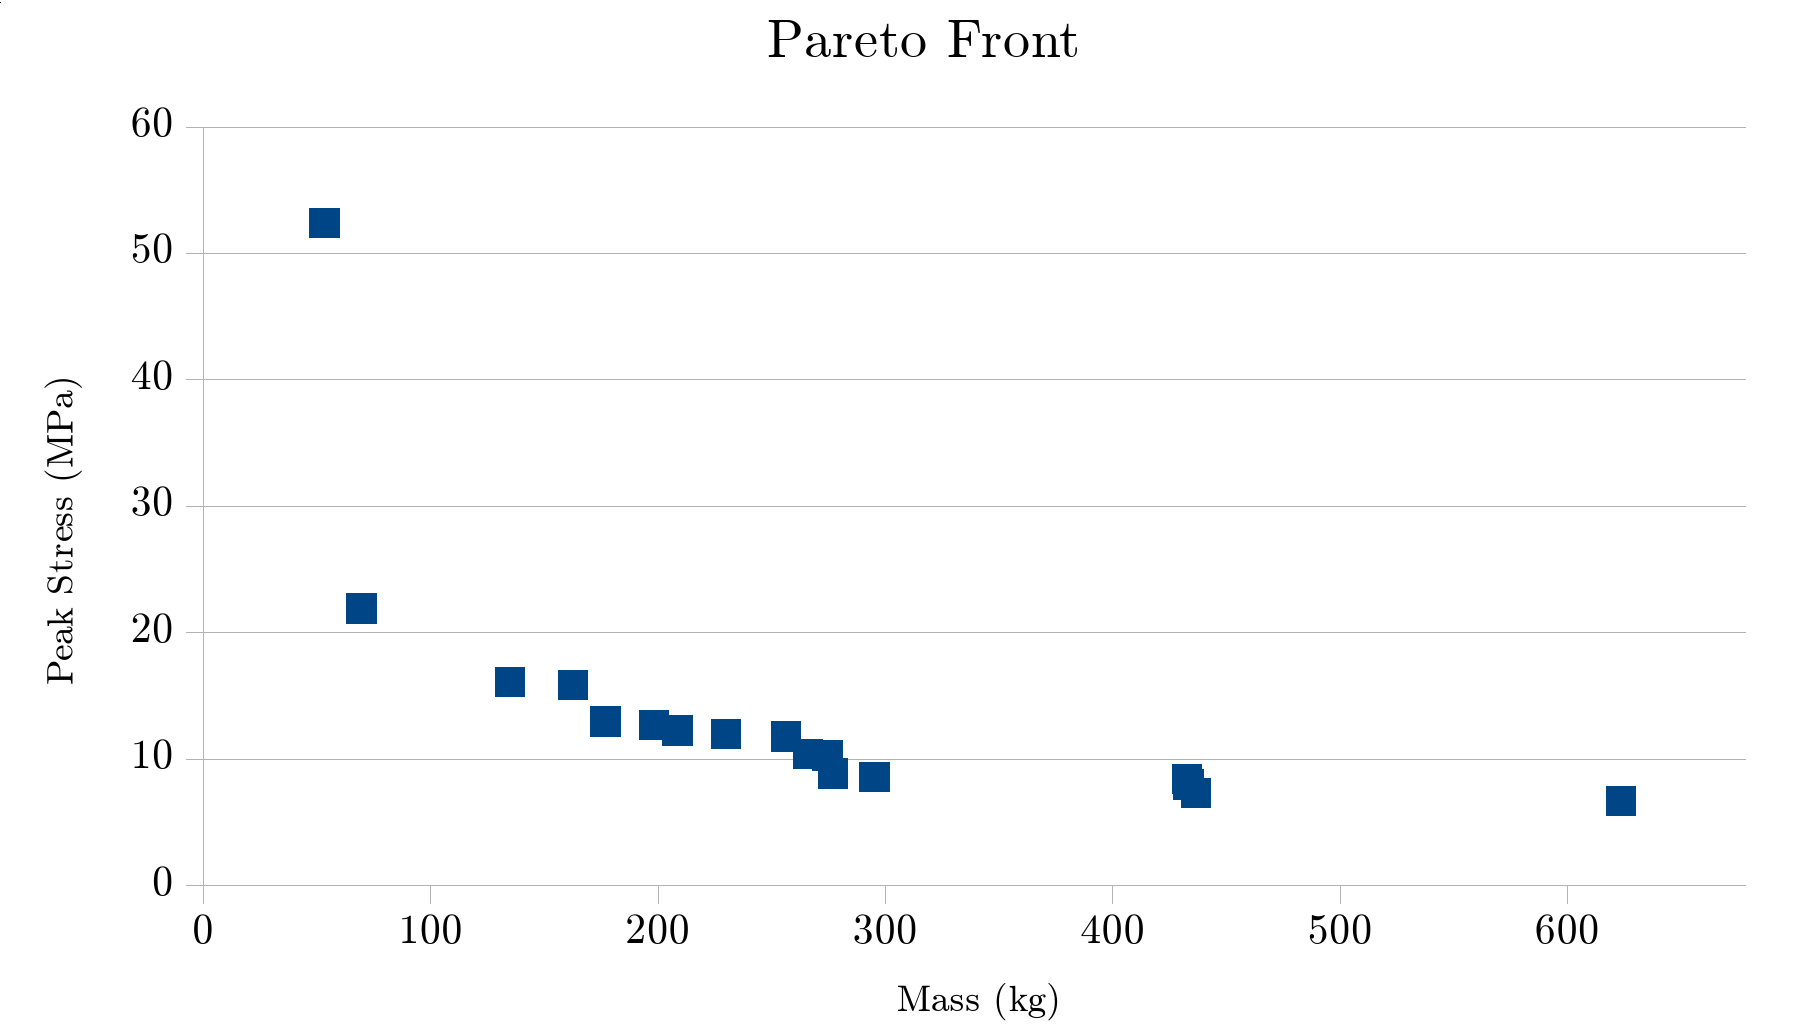
\includegraphics[width=\textwidth]{img/s2i80g200_front.png}
\caption{Graph of the Pareto Front generated through Aggregated LHS -- Same Parameters Run}
\label{fig:pfront_agg_sameparam}
\end{figure}

\subsection{Solution Statistics}
This solution also was tracked for several computing performance indicators to compare the performance of the algorithm with the other solutions. These statics are listed in Table \ref{tab:stat_agg_sameparam}. 

\begin{table}[!htbp]
  \centering
  \begin{tabular}{|l|l|}
    \hline
	  Total Generations Computed & 5000\\
    Average Time Per Generation (sec) & 19.3\\
    Total Wall Clock Time (sec)	 & 96.4E+03\\
    \hline
  \end{tabular}
  \caption{Solution Statistics for Aggregated LHS -- Same Parameters Run}
  \label{tab:stat_agg_sameparam}
\end{table}

\section{Aggregate LHS Method(Same Solution Time)}
\todo{Run this solution!!}
This solution was calculated using parameters designed to produce the same wall clock solution time as the Stochastic Loads Run. The command line that was used was:

\begin{verbatim}
python -m pystruct <<data_file>>  -S2 -i80 -g17 --csv
\end{verbatim}

\noindent Where: 

\begin{itemize}
  \item \codeword{-S2}: Select solution 2: Aggregate LHS method
  \item \codeword{-i80}: Use a population size of 80. 
  \item \codeword{-g17}: Use a generation count of 17. 
  \item \codeword{--csv}: Generate CSV output for final Pareto Front
\end{itemize}

\subsection{Resultant Pareto Front}
